\documentclass{beamer}
\usepackage[ngerman]{babel}
\usepackage[T1]{fontenc}
\usepackage[utf8]{inputenc}
\usepackage{amsmath}

\title{Privacy Preserving Record Linkage on Flink}

\subtitle{Big Data Praktikum}

\author{T. Hornoff \and M. Franke}

\institute{Abteilung Datenbanken \\ Institut für Informatik \\ Fakultät für Mathematik und Informatik \\ Universität Leipzig}

\date{04.08.2016}

\AtBeginSection[]
{
  \begin{frame}
    \frametitle{Inhalt}
    \tableofcontents[currentsection]
  \end{frame}
}

\begin{document}

	\frame{\titlepage}

	% ------------- Einleitung -------------- %
	\section[Section]{Einleitung}
    
    \begin{frame}
    		\frametitle{Privacy Preserving Record Linkage (PPRL)}        
         \begin{itemize}
         		\item Auffinden von gemeinsam genutzten Datenelementen (Korrespondenzen)
         		\item Verbindung von Datensätzen aus einer oder mehreren Datenquellen
         		\item Herausforderungen
                \begin{itemize}
                    \item Schutz personenbezogener Daten
                    %\item Sicherung der Privatspähre, des Datenschutzes \& der Vertrauchlichkeit
                    \item Wachsende Datenmengen (Skalierbarkeit)
                    \item Qualität der Daten
                \end{itemize}
         		\item Zahlreiche Anwendungsgebiete
                \begin{itemize}
                    \item Gesundheitsfürsorge
                    \item Betrugserkennung
                    \item Finanzinstitutionen \& Banken
                    \item Unternehmensanwendungen
                \end{itemize}
         \end{itemize}
    \end{frame}
    
    \begin{frame}
    		\frametitle{Apache Flink}
            %\begin{itemize}
                %%\item Analyse von Batch- und Streaming-Daten
                %\item Java und Scala
                %\item MapReduce vs. Parallel Database Systems
            %\end{itemize}
            \begin{figure}[H]
                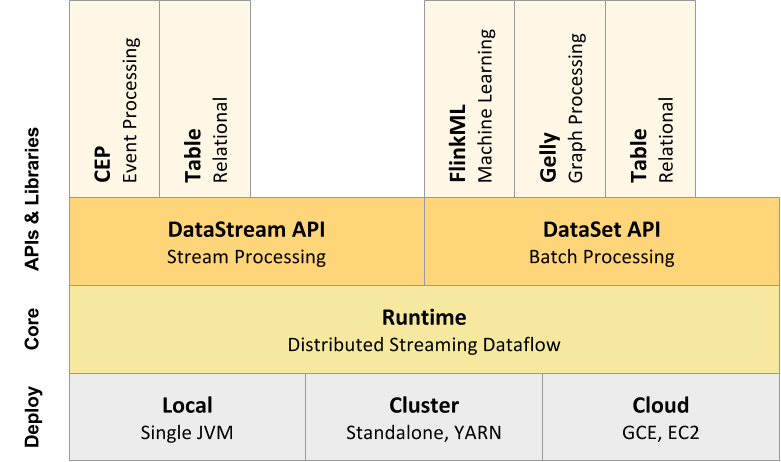
\includegraphics[width=\textwidth]{graphics/flink_stack.png}
                \caption{https://flink.apache.org/img/flink-stack-frontpage.png}
            \end{figure}
    \end{frame}
    
       % ------------- Realisierung ----------- %
    \section[Section]{Realisierung}
    
    \begin{frame}
    		\frametitle{Prozess}
    		\begin{figure}[H]
    			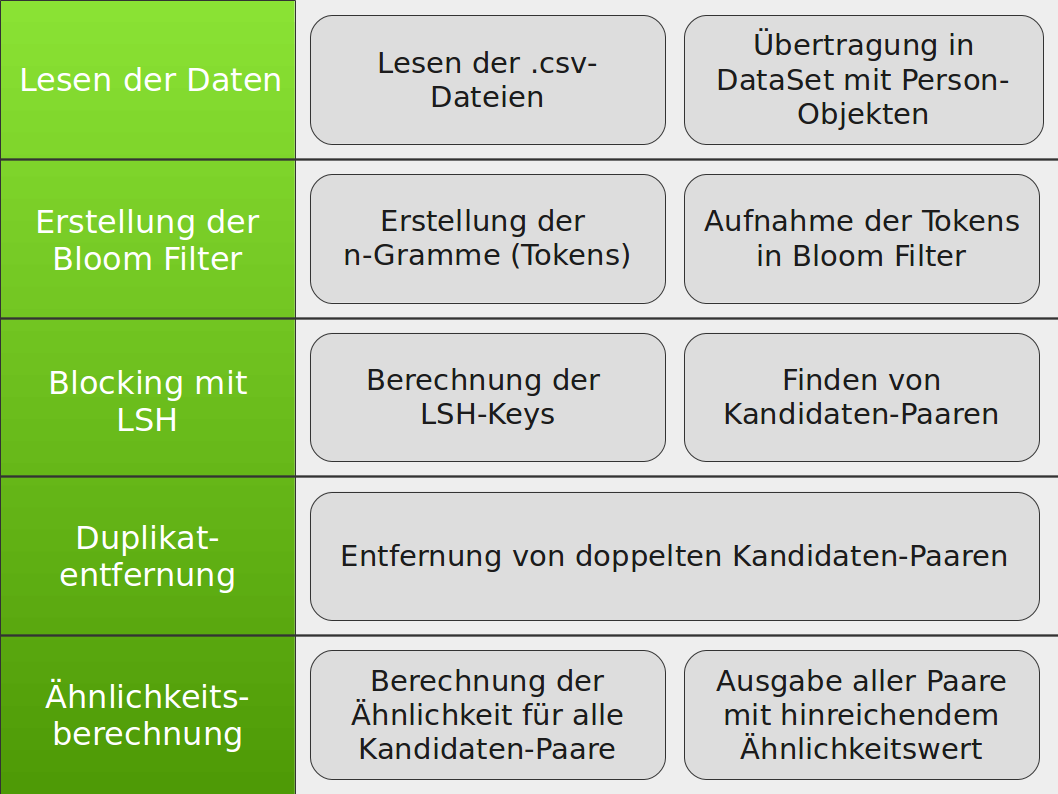
\includegraphics[width=\textwidth]{graphics/process.png}
    		\end{figure}
    \end{frame}
    
    \begin{frame}
    		\frametitle{Prozess - Lesen der Daten}
    		\begin{figure}[H]
    			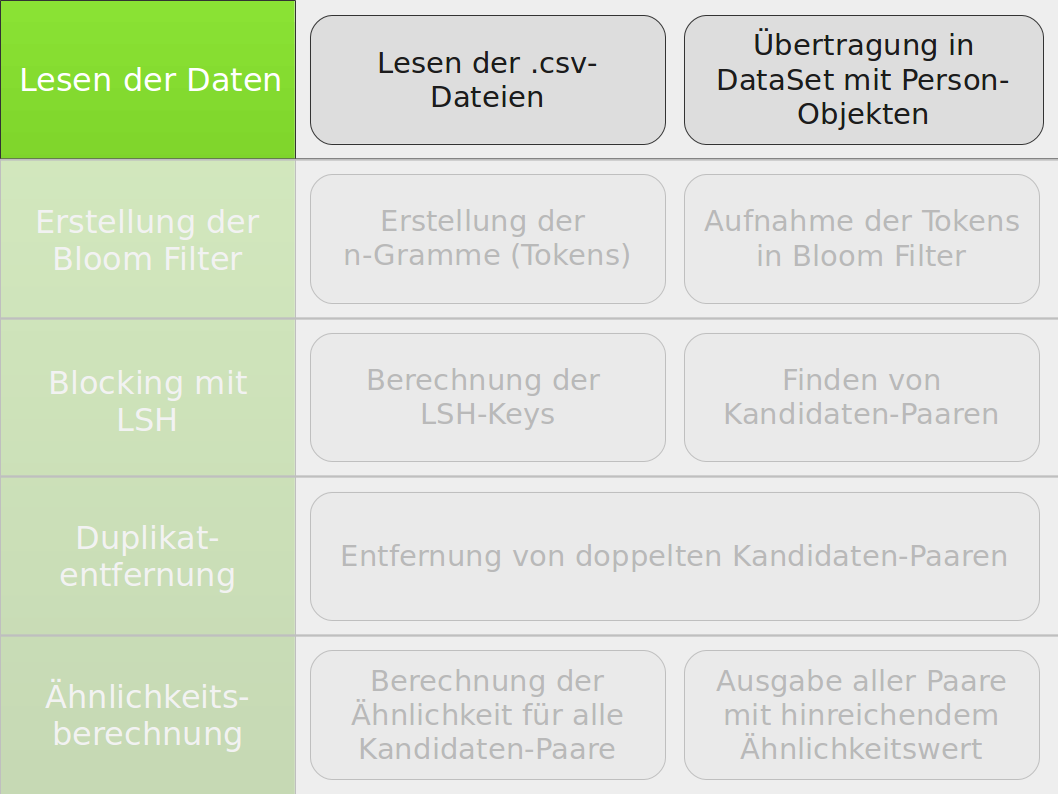
\includegraphics[width=\textwidth]{graphics/process_1.png}
    		\end{figure}
    \end{frame}
    
    \begin{frame}
    		\frametitle{Prozess - Lesen der Daten}
    		\begin{itemize}
    			\item Nutzung verschiedener Datensätze
    			\begin{itemize}
    				\item North Carolina Voter Registration Database
    					\footnote{\cite{NorthCarolinaVoterRegistration}}
    				\begin{itemize}
    					\item Erreichbar unter \url{http://dl.ncsbe.gov/}
    					\item Verschieden große Datensätze
    					\item Personenbezogene Daten (z.B. Name, Adresse, Alter, Geschlecht, ...)
    				\end{itemize}
    				\item Nutzung von generierten Daten
    				\begin{itemize}
    					\item Beginn der Übersetzung eines DataCorruptors\footnote{\cite{DataCorruptor}} in Java mit Flink 
    				\end{itemize}	
    			\end{itemize} 
    		\end{itemize}
    \end{frame}
    
    \begin{frame}
    		\frametitle{Prozess - Lesen der Daten}
    		\begin{itemize}
    			\item Aufbau des Datensatzes
    			\begin{figure}
    				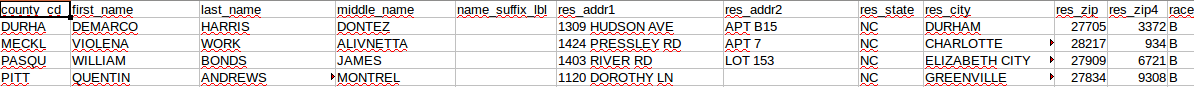
\includegraphics[width=0.95\textwidth]{graphics/voter_dataset.png}
    			\end{figure}
    		\end{itemize}
    \end{frame}
    
    \begin{frame}
    		\frametitle{Prozess - Lesen der Daten: Ergebnis}
    		\begin{itemize}
    				\item Ausgabe der Person-Objekte in der Form $(Person)$
    				\begin{figure}[H]
    					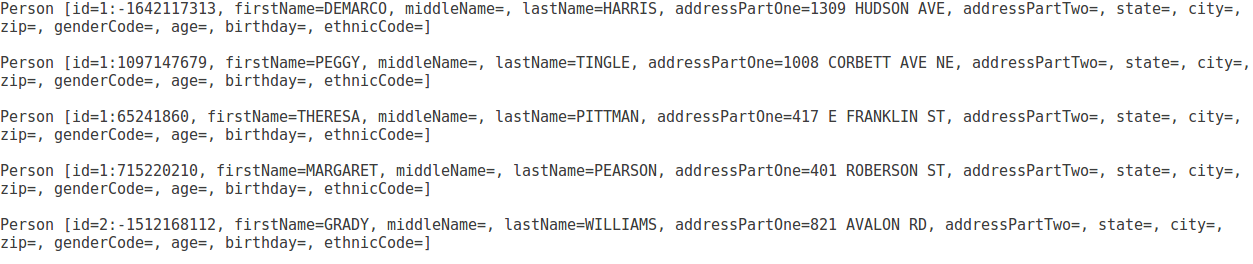
\includegraphics[width=0.95\textwidth]{graphics/persons.png}
    				\end{figure}
    		\end{itemize}
    \end{frame}
    
    \begin{frame}
    		\frametitle{Bloom Filter}
            \begin{figure}[H]
                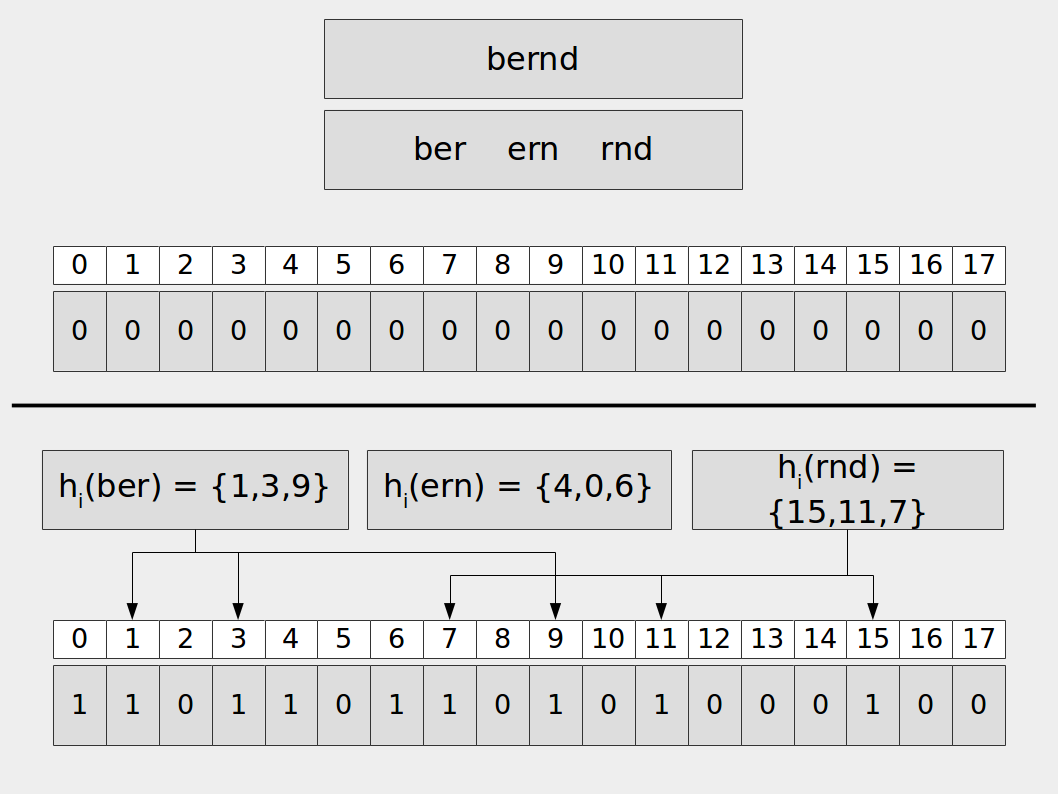
\includegraphics[width=\textwidth]{graphics/bloom_qgram.png}
            \end{figure}
    \end{frame}

    \begin{frame}
    		\frametitle{Prozess - Erstellung der Bloom Filter}
    		\begin{figure}[H]
    			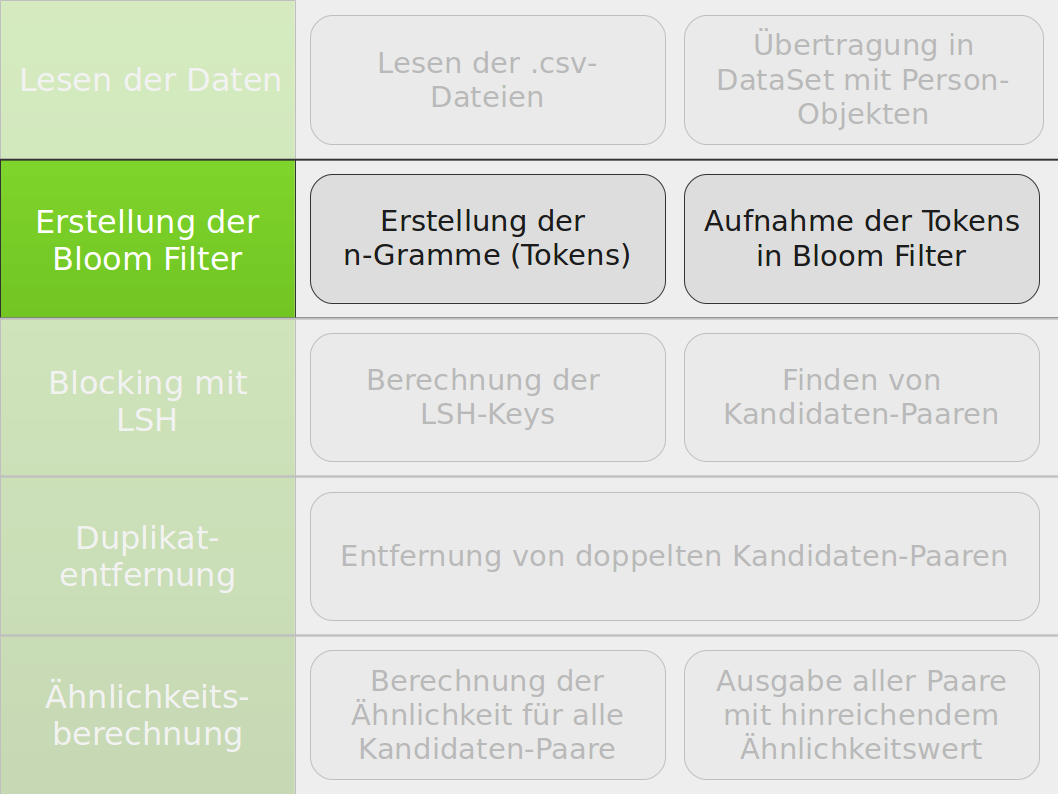
\includegraphics[width=\textwidth]{graphics/process_2.png}
    		\end{figure}
    \end{frame}
    
    \begin{frame}
    		\frametitle{Prozess - Erstellung der Bloom Filter}
    		\begin{itemize}
    			\item Eigene Bloom Filter Implementierung
    			\begin{itemize}
    				\item Einstellbare Länge und Anzahl der Hashfunktionen
    			\end{itemize}
    			\item 2 Arten der Parallelisierung
    			\begin{itemize}
    				\item Parallelisierung auf Record-Ebene
    				\begin{itemize}
    					\item Ausgabe der Token als Liste
    					\item Alle Tokens werden gemeinsam in einen Bloom Filter aufgenommen
    				\end{itemize}
    				\item Parallelisierung auf Token-Ebene
    				\begin{itemize}
    					\item Ausgabe der Tokens einzeln
    					\item Für jeden Token wird ein eigener Bloom Filter erstellt
    					\item Entstandene Bloom Filter werden durch OR-Verknüpfung vereinigt
    				\end{itemize}
    			\end{itemize}
    		\end{itemize}
    \end{frame}
    
    \begin{frame}
    		\frametitle{Prozess - Erstellung der Bloom Filter: Ergebnis}
    		\begin{itemize}
    			\item Ausgabe der Tokens in der Form $(ID_{Person}, Token)$
    				\begin{figure}[H]
    					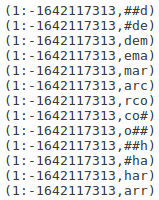
\includegraphics[width=0.18\textwidth]{graphics/tokens_1.png}
    				\end{figure}
    			\item Ausgabe der Tokens bei Parallelisierung auf Record-Ebene in der Form
    			$(ID_{Person}, List(Token))$
    				\begin{figure}[H]
    					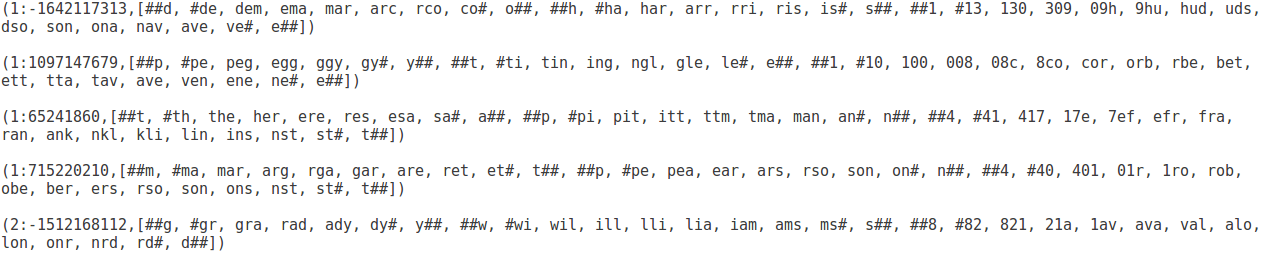
\includegraphics[width=0.9\textwidth]{graphics/tokens_2.png}
    				\end{figure}
    		\end{itemize}
    \end{frame}
   
    \begin{frame}
    		\frametitle{Prozess - Erstellung der Bloom Filter: Ergebnis}
    		\begin{itemize}
    			\item Ausgabe der Bloom Filter in der Form $(ID_{Person}, BloomFilter)$
    				\begin{figure}[H]
    					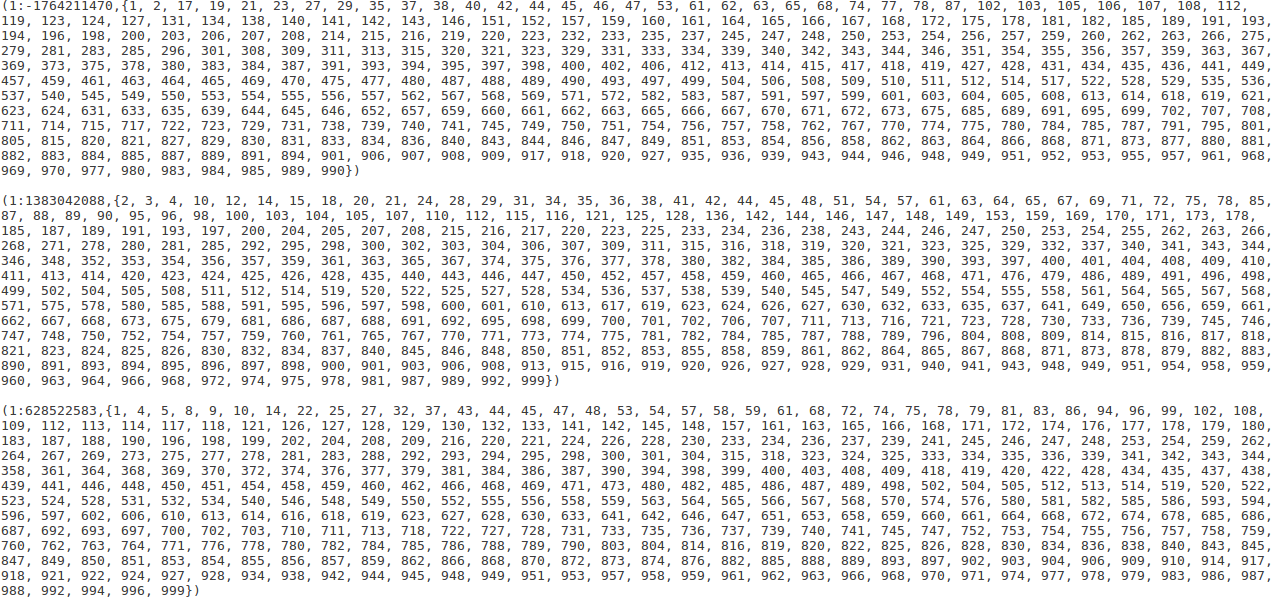
\includegraphics[width=0.9\textwidth]{graphics/bloomfilter.png}
    				\end{figure}
    		\end{itemize}
    \end{frame}

    \begin{frame}
        \frametitle{Locality Sensitive Hashing (LSH)}
       
            \begin{itemize}
                \item Jaccarrd-LSH
                    \begin{itemize}
                        \item $Jaccard(I,J) = \frac{|I \cap J|}{|I \cup J|}$
                    \end{itemize}
                \item Hamming-LSH
                    \begin{itemize}
                        \item $Hamming(I,J) = I \oplus J$
                    \end{itemize}
            \end{itemize}

    \end{frame}

    \begin{frame}
    		\frametitle{Prozess - Blocking mit LSH}
    		\begin{figure}[H]
    			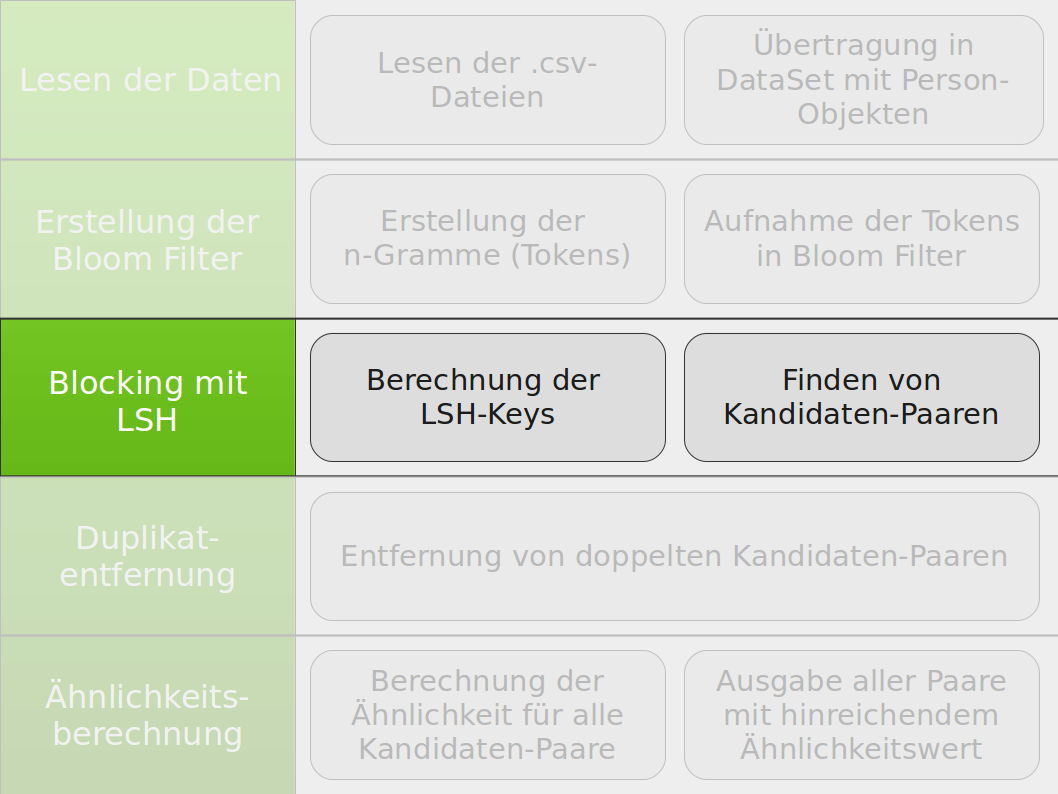
\includegraphics[width=\textwidth]{graphics/process_3.png}
    		\end{figure}
    \end{frame}
    
    \begin{frame}
    		\frametitle{Prozess - Blocking mit LSH: Ergebnis}
    		\begin{itemize}
    			\item Ergebnis des Blockings in der Form $(ID_{LshKey}, Value_{LshKey},
    			 BloomFilter)$
    		\end{itemize}
    		\begin{figure}[H]
    			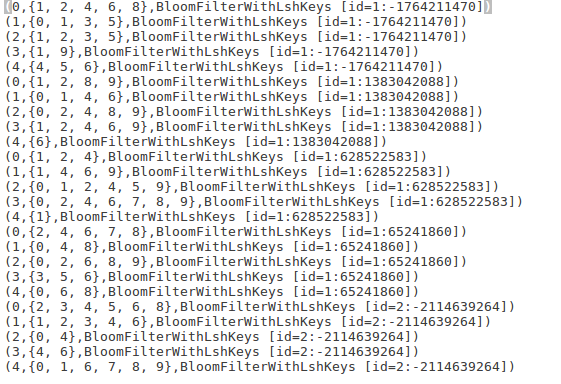
\includegraphics[width=0.8\textwidth]{graphics/lsh.png}
    		\end{figure}
    \end{frame}
    
    \begin{frame}
    		\frametitle{Prozess - Duplikatentfernung}
    		\begin{figure}[H]
    			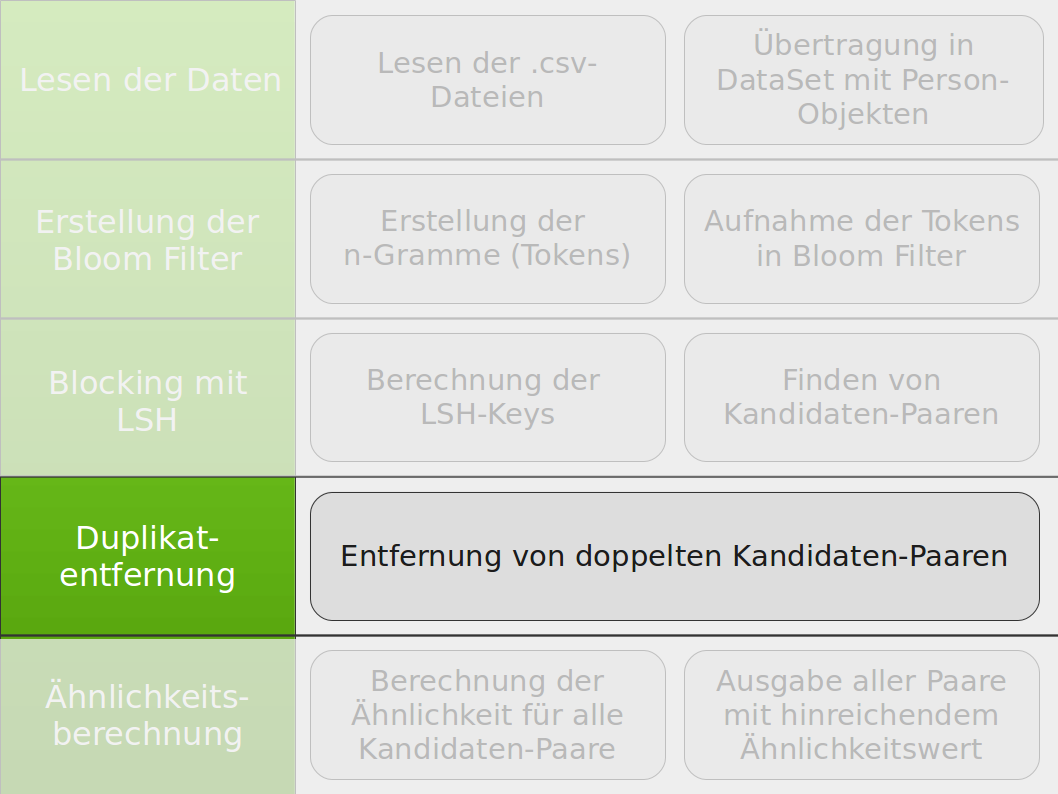
\includegraphics[width=\textwidth]{graphics/process_4.png}
    		\end{figure}
    \end{frame}
    
    \begin{frame}
    		\frametitle{Prozess - Ähnlichkeitsberechnung}
    		\begin{figure}[H]
    			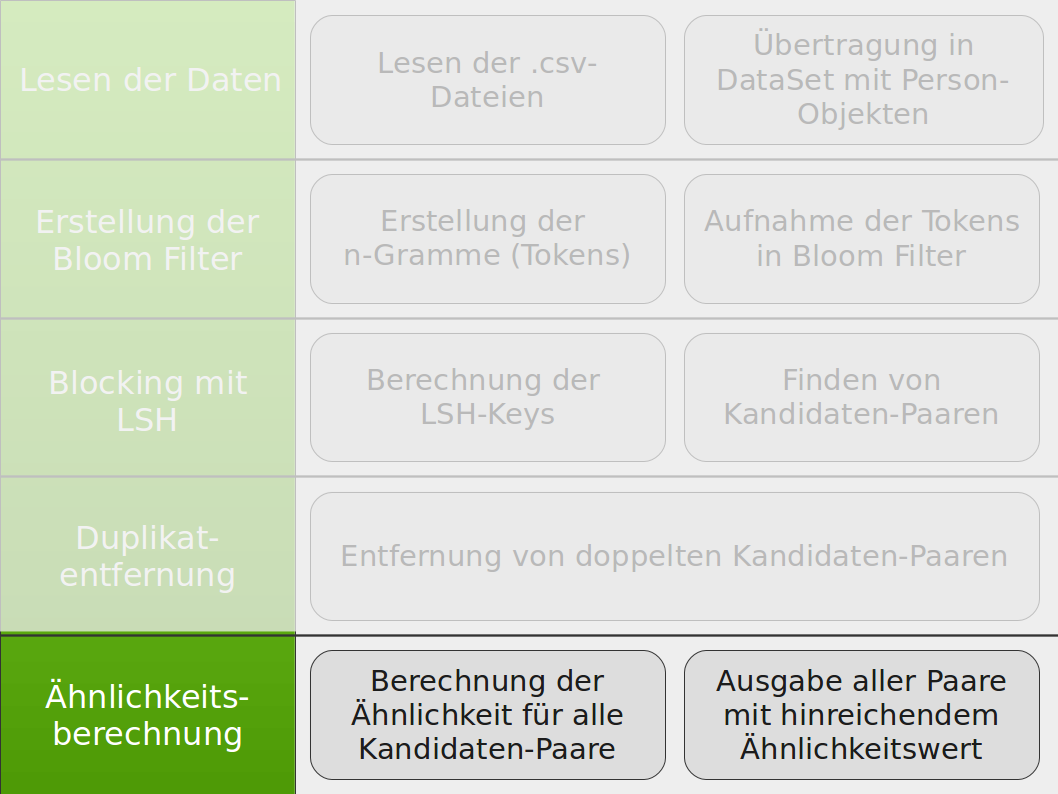
\includegraphics[width=\textwidth]{graphics/process_5.png}
    		\end{figure}
    \end{frame}
    
    \begin{frame}
    		\frametitle{Prozess - Ähnlichkeitsberechnung: Ergebnis}
    		\begin{itemize}
    			\item Ergebnis ist Matching Pair in der Form $(ID_1, ID_2)$
    		\end{itemize}
    		\begin{figure}[H]
    			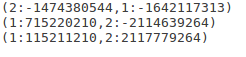
\includegraphics[width=0.5\textwidth]{graphics/endresult.png}
    		\end{figure}
    \end{frame}
    
   % ------------- Diskussion ----------- %
    \section[Section]{Diskussion}
    
    \begin{frame}
    		\frametitle{Diskussion}
    		\begin{itemize}
    			\item Vielzahl von Parametern
    			\begin{itemize}
    				\item Länge der Bloom Filter
    				\item Anzahl der Hashfunktionen
    				\item Länge der n-Gramme
    				\item Länge der LSH-Keys (\#Hashfunktionen pro Hash Family)
    				\item Anzahl der LSH-Keys (\#Hash Families)
    				\item Schwellwert für Ähnlichkeitsfunktion
    			\end{itemize}
    			\item Geeignete Auswahl der Parameter ist von großer Bedeutung
    			\begin{itemize}
    				\item Entscheidend für die Qualität und Sicherheit des PPRL
    				\item Beeinflusst Art und Weise der Parallelisierung
    			\end{itemize}
    			\item Mehrere Möglichkeiten der Parallelisierung
                \item Data Corrupter
    		\end{itemize}
    \end{frame}
     
     \begin{frame}
     	\frametitle{Quellen}
      	\bibliographystyle{alphadin}
      	\bibliography{library}
	\end{frame}
     
\end{document}
